
%(BEGIN_QUESTION)
% Copyright 2009, Tony R. Kuphaldt, released under the Creative Commons Attribution License (v 1.0)
% This means you may do almost anything with this work of mine, so long as you give me proper credit

In this process, maple syrup is heated as it passes through a steam heat exchanger, then enters an evaporator where the water boils off.  The purpose of this is to raise the sugar concentration of the syrup, making it suitable for use as a food topping.  A level control system (LT, LIC, and LV) maintains constant syrup level inside the evaporator, while an analytical control system (AT, AIR, AC, and AV) monitors the sugar concentration of the syrup and adjusts steam flow to the heat exchanger accordingly.

$$\includegraphics[width=15.5cm]{i04390x01.eps}$$

Suppose the steam boiler is having problems, causing the steam supply temperature to be less than what it normally is.  Describe in detail the effect this boiler system problem will have on the performance of the analytical control system.

\vskip 20pt \vbox{\hrule \hbox{\strut \vrule{} {\bf Suggestions for Socratic discussion} \vrule} \hrule}

\begin{itemize}
\item{} Identify as many {\it loads} in this process as you can, determining the direction of influence each one has on each controlled variable.
\item{} Suppose the heat exchanger begins to ``foul'' with solid deposits from the raw syrup, impeding the tranfer of thermal energy from the steam to the syrup.  How would the control system respond to this process change?  How could this problem be diagnosed without disassembling the exchanger?
\end{itemize}

\underbar{file i04390}
%(END_QUESTION)





%(BEGIN_ANSWER)

The analytical control system should still be able to maintain sugar concentration at setpoint, unless the steam temperature is so low that even a wide-open steam valve does not heat the incoming syrup enough to sufficiently concentrate it.

\vskip 10pt

Follow-up question: suppose the steam temperature really is this low, but we cannot fix the boiler with the tools we have available.  What would you recommend the operator do to help make this system produce on-spec syrup?

%(END_ANSWER)





%(BEGIN_NOTES)

The operator could reduce the incoming feed rate to allow the lower-temperature steam to sufficiently heat the incoming syrup.

%INDEX% Basics, control loop troubleshooting: determining effect of specified fault(s)
%INDEX% Process: maple syrup concentration (single-effect evaporator)

%(END_NOTES)


